\subsection{Use a familiar and obvious user interface}

Your system should have an familiar, simple, fluid interface, with a logical navigation structure.

By using user interface techniques that your user is already familiar with, you minimize the learning time required.
In addition there are many standard visual devices to which the user is already accustomed e.g. a magnifying glass is a familiar symbol for searching.
By reusing this icon the user will quickly know what function that performs, so it makes no sense to design a brand new icon.
If a calendar is used for the selection of dates, it doesn't make sense to use an hourglass, this will just be confusing for the user.\\

A simple interface is one shorn of unnecessary ornamentation. In particular effects such as transparency, blurring and needless animation.
Simple interfaces avoid distracting the user. Remember that less is more.
A complicated design, with too many colors and too many different abstract shapes will be more difficult to interpret.
Data representations shoulw be unambiguous.
Do not show information that is deceptive, or that requires time wasted in interpretation.
When representing the information include only what is truly necessary, always avoiding ornate graphics that only contribute noise to the representation.\\

When we speak of fluidity, we refer to user-system interactions.
It is important that interactions be like a two-way conversation, and that you let the user know that the system is responsive.
Each action that the user performs should be clearly acknowledged e.g. by some change in a color, or a spinning wheel icon, and the results should be delivered in less than five seconds.
Long waits for responses are interpreted by the user as system failure.\\
    
Using a logical navigation structure encourages the user to fully utilize the data you are providing, and reduces frustration.
It is important to give the user a degree of flexibility, that is, to enable them to make their own selections to be find the data that interests them.\\

\subsubsection*{Suggested strategies} 

\begin{itemize}
    \item Avoid complicated representations, aim for familiarity and intuitiveness.

    \item Ensure that all interface elements are easy to recognize.
    
    \item Use a logical, regular navigational structure.
\end{itemize}

\subsubsection*{In the context of Aire Guru \ldots}

Aire Guru uses an interpretation of Google's Material Design, which is very clean, without borders or decorations.
We chose a range of blue shades in combination with white and gray to evoke a relaxed atmosphere.
Importantly, we've taken care that all text has a good level of contrast with the background, so that it is easy to read.
The graphics have been designed in 2D, since they are easier to interpret and we lack the ambiguity that can occur when using depth as a measure.\\

Aire Guru consists of multiple sections, and the workflow both within and between the different sections was explicitly modeled.
The representation follows a logical sequence.
By selecting a point on the map, we will show detailed information for this point.
The next section filters the information according to the preferences of the user and lastly, it shows the history of pollutants since 2018 and the history of the pollution to which the user has been exposed.\\

We use repeated structures, and the same style, colors and iconography are used throughout the design so that the user can quickly become familiar with how it works, and can
concentrate on the meaning of the data, rather than being distracted by trying to figure out what to do.
We use GoogleMaps controls because users are already familiar with both the representation and the interactive controls.
We use clouds to represent air quality measurements, accompanied by a heart if the quality is good, by an exclamation mark if it is poor, by a cross if it is bad, and we change to a gas mask if the state is unhealthy.\\

% It is expected that the user will be interested in the level of pollution to which they are exposed in real time.
% Therefore, for users that are identified and agree to share their location, Aire Guru will show the pollution directly at the point where they are.\\

\begin{figure}[ht]
    \centering
    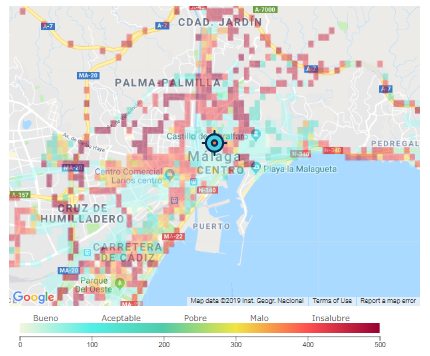
\includegraphics[width=8cm]{myLocation}
    \caption{My Location}
\end{figure}

% For maximum flexibility, the user can see the state of the air pollution by dates.
% Intermediate filtering can be done both by medical conditions and by pollutants.
% Finally, in the lower area where we have the historical data by area and personalization, we can visualize the information with different levels of detail; time, day, month and year.
% We can also select the date we want.\\

% \begin{figure}[ht]
%     \centering
%     \subfigure[Date filter]
%         {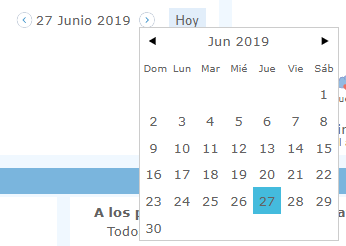
\includegraphics[width=5.5cm]{dateFilter}}
%     \hfill
%     \subfigure [Medical conditions filter]
%         {\includegraphics[width=5.5cm]{MedicalConditionFilter}}
%     \vfill
%     \subfigure[Pollutants filter]
%         {\centering 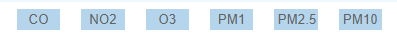
\includegraphics[width=6cm]{pollutantsFilter}}
%     \caption{Filters}
% \end{figure}

Due to the large amount of data that is offered to the user, a waiting icon has been implemented to indicate that the website is processing information.
Each time a control is pressed on the page, it is indicated with a change of color tonality.
In addition, progressive transitions are used to indicate a process is happening.\\

\begin{figure}[ht]
    \centering
    \subfigure[Searching bar]
        {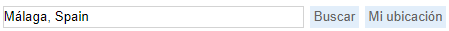
\includegraphics[width=5.5cm  ]{searchingBar}}
    \hfill
    \subfigure [Tabs]
        {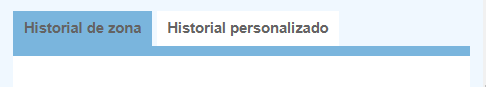
\includegraphics[width=5.5cm]{tabs}}
    \vfill
    \subfigure[Link]
        {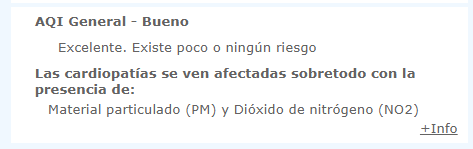
\includegraphics[width=6cm]{link}}
    \hfill
    \subfigure [Waiting symbol]
        {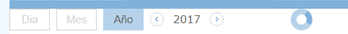
\includegraphics[width=5.5cm]{waitingSymbol}}
    \caption{Standard widgets}
\end{figure}